\scanpage{77}
/ op. hermitiens positifs, enfin satisfait à la formule (12).

\margin{\uline{Mettre en tête 2 et corollaire}}

\uline{Proposition 3} Soient $E$ et $F$ deux espaces de Hilbert, soient $u_i$ ($i=1,\mathord{.}\,\mathord{-}n$) des applications de Fredholm de $E$ dans $F$; alors $u_1\wedge\mathord{-}\wedge u_n$ est une application de Fredholm de $\overset{n}{\Lambda}^{(2)}E$ dans $\overset{n}{\Lambda}^{(2)}F$, et
\reversemarginpar\margin{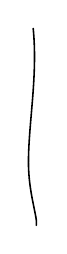
\begin{tikzpicture}[x=1mm,y=1mm,line cap=round]\draw[line width=.2mm] (.8,25) .. controls (1.4,19) and (.2,13) .. (.2,8) .. controls (.2,4) and (1.4,1) .. (1.2,0);\end{tikzpicture}}\normalmarginpar

\[
\begin{array}{@{}l@{\qquad}l@{}}
(13) & {\color{red}\boxed{\color{black}\displaystyle \lVert u_1\wedge\mathord{-}\wedge u_n\rVert_1\leq\frac1{n!}\lVert u_1\rVert_1\mathord{-}\lVert u_n\rVert_1}}
\end{array}
\]

En effet, il suffit de \deleted{\unsure{$\leq$}} vérifier \deleted{que si} si \deleted{$u_1=a_1'\otimes$} $u_i=\bar b_i\otimes a_i$, \deleted{\unsure{les} \illegible{1}} avec $\lVert\bar b_i\rVert\leq1$, $\lVert a_i\rVert\leq1$, alors $\lVert u_1\wedge\mathord{-}\wedge u_n\rVert_1\leq1/n!$, \deleted{\unsure{car}} puisqu'alors il existe une application \unsure{$n$ fois|de Ban} linéaire \deleted{\unsure{continue}} \inserted{de norme $\leq1/n!$} de $(\bar E\widehat{\otimes}E)^n$ dans \deleted{\unsure{dans}} $\bar F\widehat{\otimes}F$ (où $F=\overset{n}{\Lambda}^{(2)}E$) qui coïncide avec \inserted{$(u_1,\mathord{.}\,\mathord{-}u_n)\longrightarrow$} $u_1\wedge\mathord{-}\wedge u_n$ pour des $u_i$ décomposables, donc partout puisque les deux applications sont continues \deleted{\unsure{par}} en \deleted{\unsure{tant}} qu'applications, dans $L(F)$.

Or pour $u_i=\bar b_i\otimes a_i$, on a

\[
\deleted{\unsure{\overset{n}{\Lambda}}}\quad u_1\wedge\mathord{-}\wedge u_n=\frac1{n!}(\bar b_1\wedge\mathord{-}\wedge\bar b_n)\otimes(a_1\wedge\mathord{-}\wedge a_n),
\]

\inserted{(voir Chap I, N\textsuperscript{o} 1, formule (8))} d'où

\[
\lVert u_1\wedge\mathord{-}\wedge u_n\rVert_1\leq\frac1{n!}\lVert\bar b_1^c\wedge\mathord{-}\wedge\bar b_n\rVert\,\lVert a_1\wedge\mathord{-}\wedge a_n\rVert\leq\frac1{n!}\prod\lVert a_i\rVert\,\lVert\bar b_i\rVert
\]

(formule (5,), d'où (13).

\uline{Corollaire 1} Soit $E$ un espace de Hilbert, et \deleted{\unsure{$u$}}\inserted{$u,u_i$} $\in L^1(E;E)$ \inserted{$(i=1,\mathord{-} n)$} \deleted{des} opérateurs de Fredholm dans $E$. Alors $\overset{n}{\Lambda}u$ est un opérateur de Fredholm dans $\overset{n}{\Lambda}^{(2)}E$, et on a
\reversemarginpar\margin{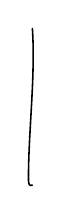
\begin{tikzpicture}[x=1mm,y=1mm,line cap=round]\draw[line width=.2mm] (.7,20) .. controls (1.1,14) and (.2,7) .. (.2,1) .. controls (.2,.1) and (.3,0) .. (.7,.1);\end{tikzpicture}}\normalmarginpar

\[
\begin{array}{@{}l@{\qquad}l@{\quad}l@{}}
(14) & \deleted{\unsure{\text{alors}}}\ \deleted{\unsure{\alpha_n(u)}}{\color{red}\boxed{\color{black}\displaystyle\left\{\begin{aligned}
\alpha_n u_1,\mathord{-}u_n)&=\operatorname{Tr}u_1\wedge\mathord{-}\wedge u_n)\\
\alpha_n(u)&=\operatorname{Tr}(\overset{n}{\Lambda}u)
\end{aligned}\right.}} & \begin{array}{@{}l@{}}\strut\\\text{en particulier}\end{array}
\end{array}
\]

(où $\alpha_n(u)$ est ${\color{red}\overline{\color{black}\text{défini dans}}}$ Chap 1, \S~2, prop 1) En effet, $(14)_{\unsure{2}}$ est vraie \deleted{pour \unsure{tout}} quand on

\margin{78}
